\chapter[Plotting the PSD of the Ensemble]{Plotting the PSD of the Ensemble}
\label{cp:plotting-the-psd-of-the-ensemble}

To plot the Power Spectral Density (PSD) of the ensemble, we first created a
function that can do the same things as this equation we were taught in
\cite{DigitalCommunicationsLecture4}:

\begin{equation}
    \label{eq:PSD}
    S_X(f) = \mathcal{F}\{R_X(\tau)\}
\end{equation}

The theoretical PSDs for each line code are derived as:

\begin{equation}
    \label{eq:PSD_polar_nrz}
    S_x(f)\big|_{\text{Polar NRZ}} = A^2 T \, \text{sinc}^2(\pi f T)
\end{equation}

\begin{equation}
    \label{eq:PSD_unipolar_nrz}
    S_x(f)\big|_{\text{Unipolar NRZ}} = \frac{A^2 T}{4} \, \text{sinc}^2(\pi f T)
    + \frac{A^2}{4}\,\delta(f)
\end{equation}

\begin{equation}
    \label{eq:PSD_polar_rz}
    S_x(f)\big|_{\text{Polar RZ}} = \frac{A^2 T}{4} \,
    \text{sinc}^2\!\left(\frac{\pi f T}{2}\right)
\end{equation}

\begin{listing}[H]
    \caption{PSD Calculation Function}
    \label{listing:PSDCalculationFunction}
    \begin{minted}{matlab}
function [PSD_sim, PSD_theo] = compute_psd(Rx, N_fft, center, half_len, freq, Fs, A, Tb, type)
Ts  = 1/Fs;
df  = Fs / N_fft;
f   = freq;

% Simulated PSD via FFT of zero-padded Rx
Rx_padded = zeros(1, N_fft);
Rx_padded(center-half_len : center+half_len) = Rx;
PSD_sim = fftshift(abs(fft(ifftshift(Rx_padded)))) * Ts;
end
    \end{minted}
\end{listing}

\begin{figure}[H]
    \centering
    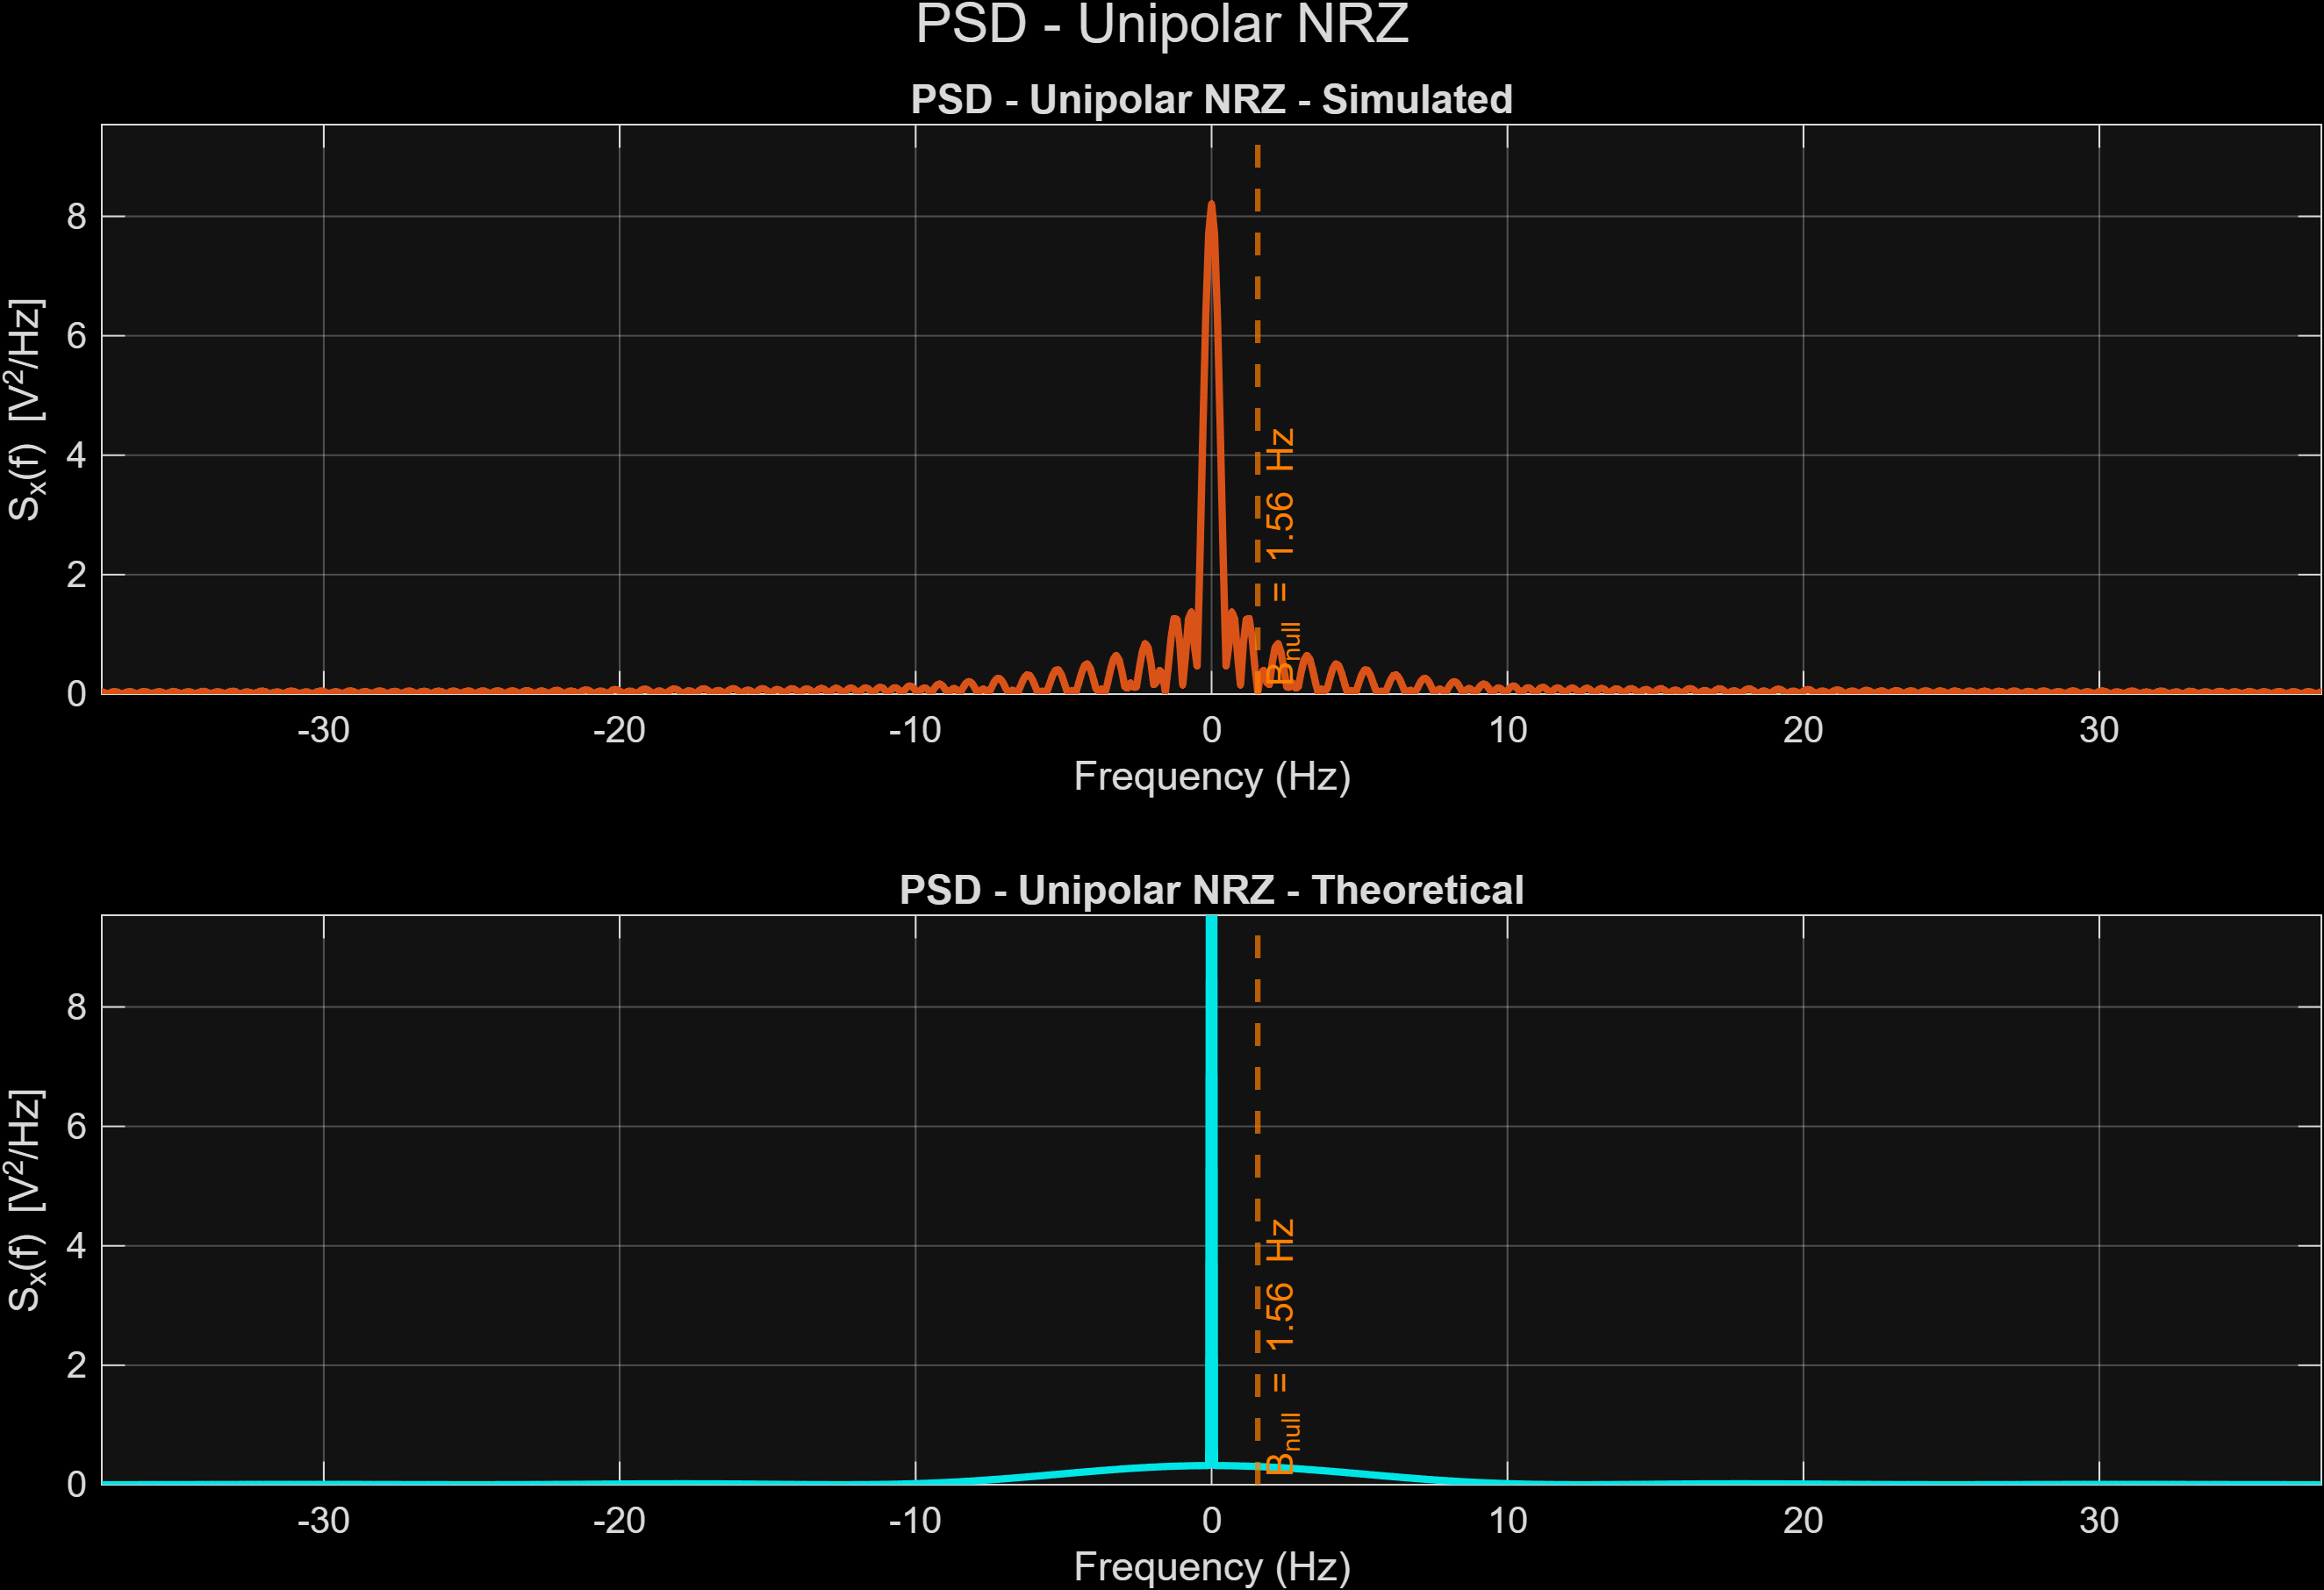
\includegraphics[width=0.48\linewidth]{Figures/PSD_-_Unipolar_NRZ_-_Theoretical.png}
    \caption[Unipolar NRZ PSD]{Unipolar NRZ PSD.}
    \label{fig:UNIPOLAR_NRZ_PSD}
\end{figure}

\begin{figure}[H]
    \centering
    \begin{minipage}{0.48\textwidth}
        \centering
        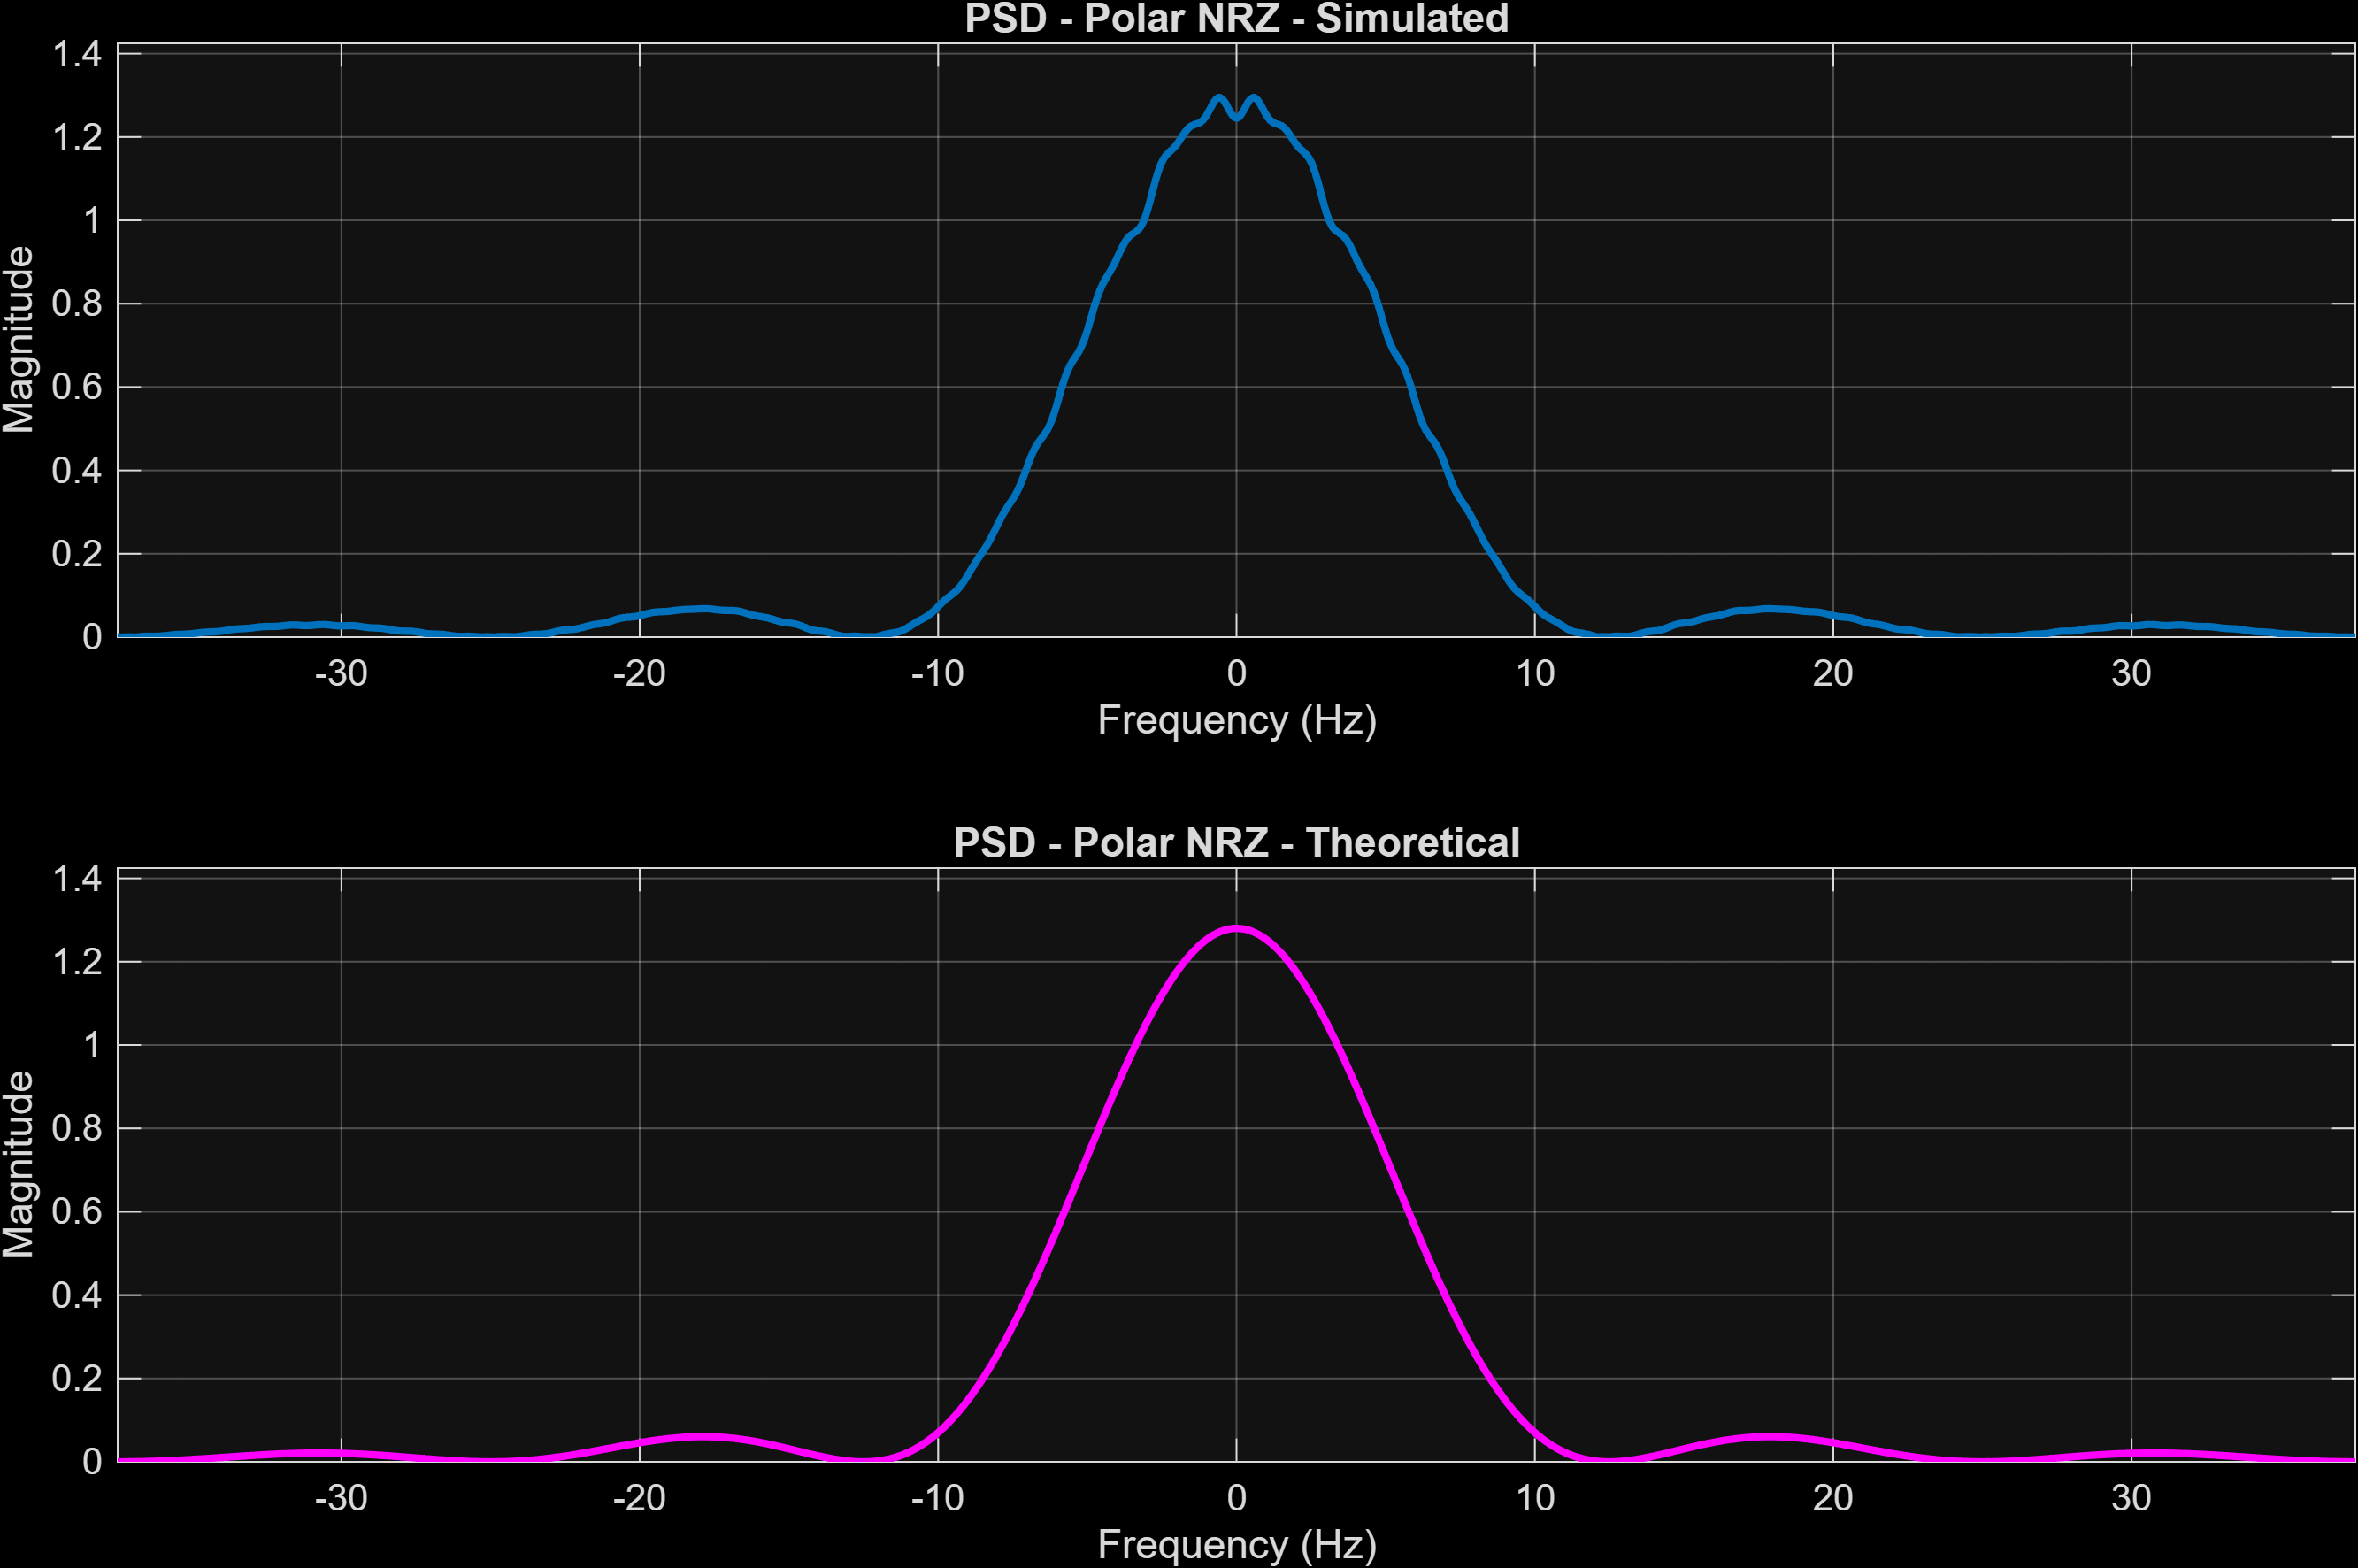
\includegraphics[width=\textwidth]{Figures/PSD_-_Polar_NRZ_-_Theoretical.png}
        \caption[Polar NRZ PSD]{Polar NRZ PSD.}
        \label{fig:POLAR_NRZ_PSD}
    \end{minipage}
    \hfill
    \begin{minipage}{0.48\textwidth}
        \centering
        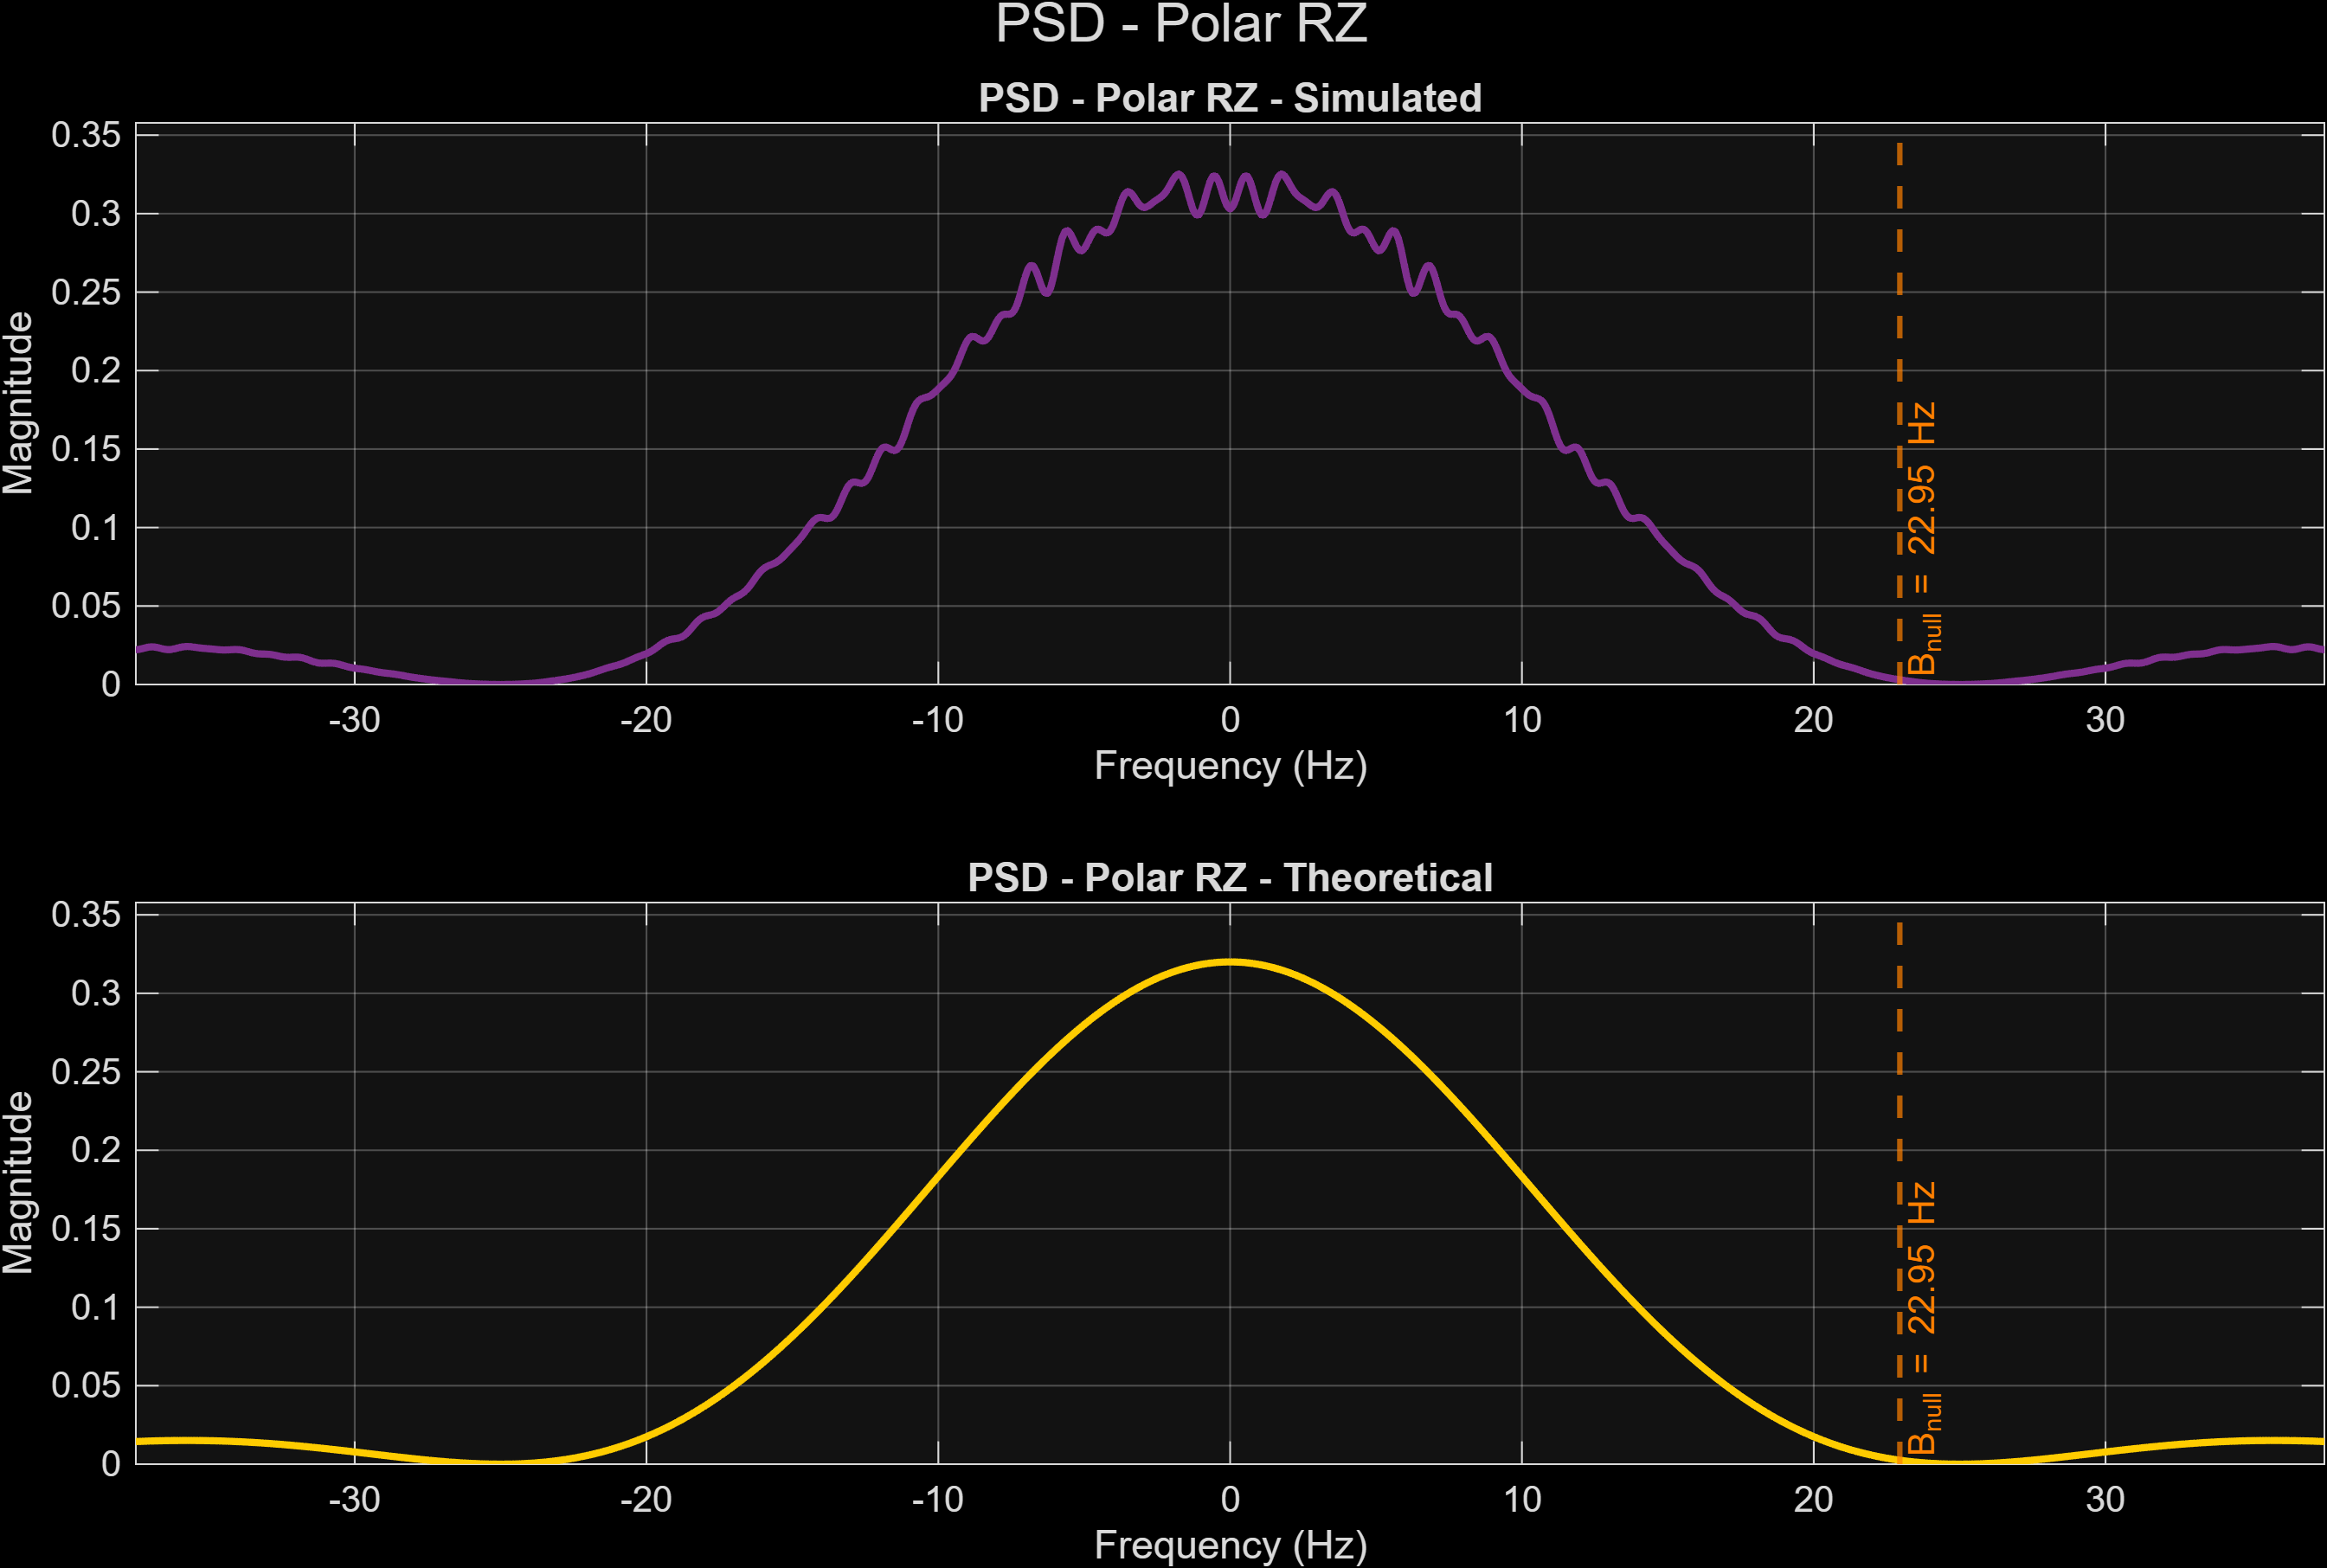
\includegraphics[width=\textwidth]{Figures/PSD_-_Polar_RZ_-_Theoretical.png}
        \caption[Polar RZ PSD]{Polar RZ PSD.}
        \label{fig:POLAR_RZ_PSD}
    \end{minipage}
\end{figure}

Observations from each graph:
\begin{itemize}
    \item \textbf{Unipolar NRZ PSD}:
          \begin{itemize}
              \item The simulated PSD closely follows the theoretical $\text{sinc}^2$ envelope
                    of \autoref{eq:PSD_unipolar_nrz}, confirming the accuracy of our calculations.
              \item The PSD has a DC spike at $f = 0$, which is expected from the $\frac{A^2}{4}\,\delta(f)$
                    term in \autoref{eq:PSD_unipolar_nrz}, since the signal has a non-zero mean.
          \end{itemize}
    \item \textbf{Polar NRZ PSD}:
          \begin{itemize}
              \item The simulated PSD closely follows the theoretical $\text{sinc}^2$ envelope
                    of \autoref{eq:PSD_polar_nrz}, confirming the accuracy of our calculations.
              \item The PSD has no DC spike, which is consistent with \autoref{eq:PSD_polar_nrz}
                    containing no $\delta(f)$ term, since the signal has a zero mean.
          \end{itemize}
    \item \textbf{Polar RZ PSD}:
          \begin{itemize}
              \item The simulated PSD closely follows the theoretical $\text{sinc}^2$ envelope
                    of \autoref{eq:PSD_polar_rz}, confirming the accuracy of our calculations.
              \item Similarly to Polar NRZ, the PSD has no DC spike since the signal is polar
                    with a zero mean. However, the wider sinc argument $(\pi f T / 2)$ in
                    \autoref{eq:PSD_polar_rz} results in a wider mainlobe, placing the first
                    null at twice the frequency compared to NRZ.
          \end{itemize}
\end{itemize}